%!TEX root = ../tommaso-thesis.tex
%!TEX spellcheck = en_US

% \chapter{State of the Art}\label{ch:related}
\coolchapter{State of the Art}{}{ch:related}

% \section{History of the Issue Tracking Systems}

Correctness is clearly an essential property for a computer program to work.
However, it is nearly impossible to determine whether a non-trivial program is really correct: the huge amount of different variables and environments that a program usually gets exposed to, makes predicting all the potentially harmful situations a task to hard to tackle.
Even if we could determine the absolute correctness of a program in a given moment in time, this does not guarantee that it will keep behaving correctly in the future: There are a number of external factors that influence the execution of a program that can cause the arise of problems that could not be observed before.
Such external factors could for example be changes in the underlying technology, like the operating system, or different usage conditions like a change of the input format.
For this reason ---since we cannot get rid of bugs--- dealing efficiently with defects is a crucial aspect in the success of a software system.

Since the beginning of the history of computer programming, developers needed a procedure to track and describe the appearance, impact, and resolution of the errors encountered during the evolution of a system.
\figref{fig:first-bug-report} shows what the folklore considers to be the first bug report, written by Grace Hopper.\seeurl{http://ei.cs.vt.edu/~history/Hopper.Danis.html}
From that handwritten paper note to present days, issue trackers evolved and adapted to reflect the different development practices introduced during the years.
This led to a well established \emph{de facto} model of a bug report.

In this chapter we illustrate the state of the art in issue tracking, providing an overview on the current tools and practices and the approaches they propose, to identify the useful elements in issue tracking.

\begin{figure}[t]
\centering
  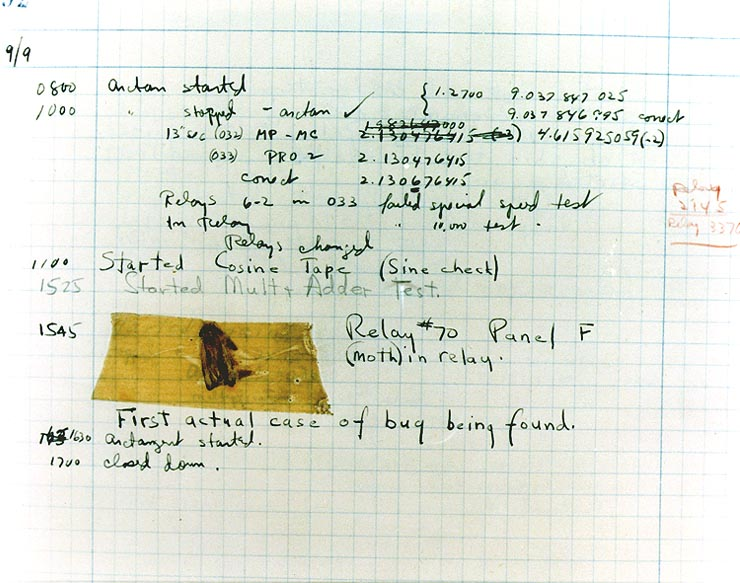
\includegraphics[width=.7\linewidth]{related/bug}
  \caption[The first "bug" report.]{This piece of paper is considered to be the first "bug" report. It was written by Grace Hopper when she was working on the Mark II computer, to document the find of a moth that caused a malfunction in the system.}
  \label{fig:first-bug-report}
\end{figure}


%%%%%%%%%%%%%%%%%%%%%%%%%%%%%%%%
\section{Issue Tracking Systems}\label{sec:related-bugtrackers}
%%%%%%%%%%%%%%%%%%%%%%%%%%%%%%%%

\begin{figure}[t]
\centering
  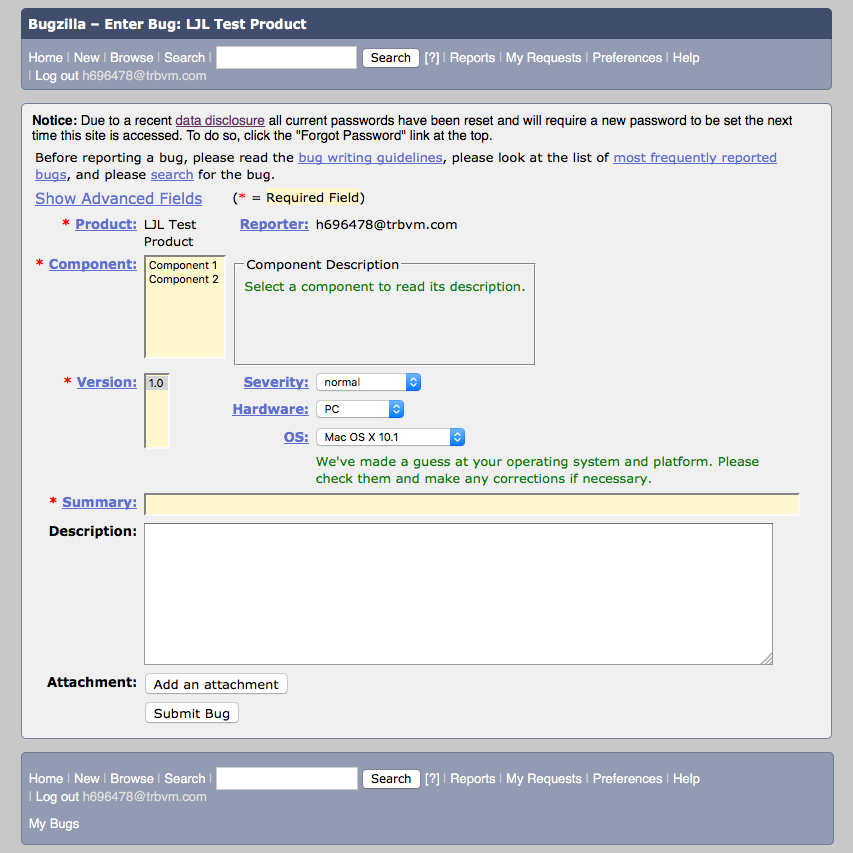
\includegraphics[width=.7\linewidth]{related/bugzilla}
  \caption{An old Bugzilla submission form}
  \label{fig:bugzilla-interface}
\end{figure}

In 1998, the Mozilla Foundation released the first version of \bzilla, which would soon become the reference issue tracking system.
During the years different alternative tools emerged, providing their own set of customizations and personalizations.
In this section we present four platforms, selected by importance and overall adoption, showing their salient features: \bzilla, \jira, the \gth issue tracker and \fbz.


\subsubsection{Bugzilla}
\bzilla\seeurl{https://www.bugzilla.org} is one of the oldest and most popular issue tracking systems, that inspired many existing issue trackers. Developed by the Mozilla Foundation, it is used by several open source projects, as well as industrial customers. \bzilla allows its users to obtain a great level of detail in specifying an issue producing, however, a complex interface.
\figref{fig:bugzilla-interface} shows the interface that \bzilla used to have in one of its previous versions.


\subsubsection{Jira}
\jira\seeurl{https://www.atlassian.com/software/jira} by Atlassian is one of the most famous commercial issue trackers, used by Twitter, Linkedin, and Ebay. It provides a polished interface and strong integration with the tools developed by the company. It uses a model similar to \bzilla.

% \begin{wrapfigure}[9]{r}{0.45\textwidth}
\begin{figure}[t]
\centering
 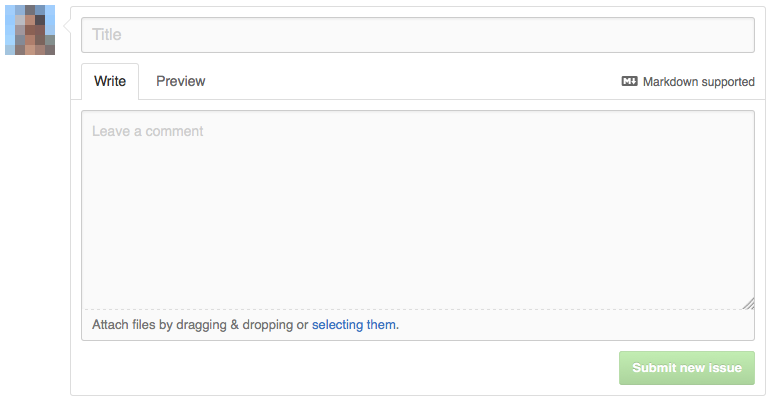
\includegraphics[width=.95\linewidth]{related/github}
 \caption{\gth bug report submission form.}
 \label{fig:github-interface}
% \end{wrapfigure}
\end{figure}

\subsubsection{GitHub}
\gth\seeurl{https://www.github.com} is a popular \texttt{Git} repository hosting service, used to develop several popular open source projects, that offers a simple issue tracker. \gth adopts a simplified model of a bug report, but offers a strong integration with the versioned source code, by linking issues with specific commits.

\subsubsection{FogBugz}
\fbz\seeurl{https://www.fogcreek.com/fogbugz} is an issue tracker developed by FogCreek. It uses a bug model similar to the one of \bzilla, slightly more polished and user-friendly, due to its clean user interface and advanced filtering capabilities. It poses a strong accent on customization, by letting users define custom filters and views.

\subsubsection{} %{Other platforms}
Together with these platform, the open source and commercial scenes provide other popular solutions, like Redmine\seeurl{https://redmine.org/} or Trac.\seeurl{http://trac.edgewall.org/}
It is however interesting to observe that, while these systems propose different degrees of integration with the tools in their ecosystem (\eg the versioning system), the fundamental approach they adopt follows the same paradigm made popular by \bzilla: a textual description with additional customizable metadata.
Further improvements to issue trackers, and the research around them, are built on top of this paradigm.
In the following sections, we present the efforts of researchers to improve issue trackers and the model of a bug report in support of the bug fixing activity.



%%%%%%%%%%%%%%%%%%%%%%%%%%%%%%%%%
\section{Visualizing Bug Reports}\label{sec:related-visualize} % was sec:related-blend
%%%%%%%%%%%%%%%%%%%%%%%%%%%%%%%%%

% \subsection{Understanding Bug Reports}

Many researchers showed how using data generated during the programming activity can provide valuable information about the evolution of a project.
For example, Bacchelli et al. proposed an Eclipse plugin to integrate email communication in the IDE~\cite{Bacc2011a}.
They showed that having the email data produced during the development of a software system at one's disposal helps supporting program comprehension tasks, such as finding entry points in a system and recovering additional documentation.
Another example has been given by Zimmermann \etal, who applied data mining techniques to version histories to detect changes and build prediction model to suggest future changes to developers~\cite{Zimm2004a}.


\subsection{Visualizations of an Issue Tracker}

Just having the raw data, however, is often not enough: to turn it into actionable knowledge it is important to build tools to make use of this information.
Reading a bug report is a difficult step in the debugging process: Browsing the large amount of information and decide whether how much to rely on the data reported by the users, consume a significative amount of developers' time.
To alleviate this burden, researchers devised a number of approaches based on the visualization of the data inside issue trackers.
For example, D'Ambros \etal performed an analysis of the \bzilla bug repository: They summarized the diagram of the state transitions of a report and proposed a set of visualizations to support the analysis of a bug database at different levels of granularity.
Their approach allows the user to navigate the history of a single issue tracker and inspect selected part of the system with customized filters and synthesized a state transitions diagram of a report~\cite{DAmb2007b}.
They built visualizations to support the analysis of a bug database at different levels of granularity, that depicts bug reports as independent entities.
Their approach allows users to browse the history of an issue tracker and inspect parts of the system with custom filters.
Knab \etal proposed visualizations to ease the understanding of the data in an issue tracker and find hidden patterns~\cite{Knab2009a,Knab2010a}.
Hora \etal proposed a visual exploration of the bug repository, considering bugs as first class entities, and linking them to other software artifacts~\cite{Hora2012a}.

All these approaches focus on retrospective analyses.
We believe that while conceptually interesting, there is little practical utility in daily development, since after all the goal of an issue tracking system is not to look at defects, but to actually fix them.
This implies that even the most elaborated techniques are of limited actionability, since the bug fixing process takes place in a different space, namely the integrated development environment (IDE).
We believe that the use for a visualization is not to simply display the data, but to establish a first-class link to the development environment.


\subsection{Visual Storytelling}

Even with the means to efficiently inspect single bug reports, getting a big picture of the data contained in an issue tracker, and how it relates to the system, is often a completely different task, as the data has to be interpreted on a different level.
To effectively present and understand such an amount of data, many researchers and practitioners adopt a \emph{Visual Storytelling} approach.
The ability of contextualizing the information in a story that explains the meaning of the data is becoming more and more central to the skills required to data scientists~\cite{Segel2010a}.

Among the different visualizations that researchers used to represent a software system, the city metaphor has proven to be effective in giving a high level picture of a group of entities, allowing the user to navigate, zoom and inspect the various components and refine the view~\cite{Wett2011a}.
This approach has been adopted in different scenarios, depicting different kind of information pertaining several steps of the development activity, such as changes in the system, the defects involving different components in the system, issues in quality checking rules or the exceptions in the system~\cite{Panas2003a}.

Other visualization approaches tried to focus on the evolution of software systems, specifically the version repositories, the dependencies or the structures.
For example, Fischer \etal~\cite{Fisch2006a} proposed \tool{EvoGraph}, an approach based on data extracted from a system release history, that visualizes the evolution of structural dependencies through 2D visual representations.
Girba \etal~\cite{Girb2005a} focused on the visualization of the evolution of class hierarchies, correlating the history of classes and their relationships, \eg inheritance.
The approach by Voinea \etal~\cite{Voin2007a} uses a combination of color and texture to represent as many attributes as possible to display information extracted from software configuration management systems.
Another important approach is the one by Ratzinger \etal~\cite{Ratz2005a}, that represents systems as nested, zoomable graphs.

However, while these approaches effectively visualize data about a single aspect that impacts or involves a system, they fall short in correlating this information with knowledge coming from diverse data sources and impacting diverse concerns.
Such additional information could effectively integrate the existing data to uncover further relations between the elements of the system.
We think that an approach that considers more than one kind of data and presents the information in a unified, uniform view, normalizing and balancing each source, could provide a greater value in understanding a software project and the activities happening in its ecosystem.



%%%%%%%%%%%%%%%%%%%%%
\section{Bug Reports}\label{sec:related-reports}
%%%%%%%%%%%%%%%%%%%%%

Dealing with bug reports is a non-trivial task, that poses a number of communication problems among users and developers.
Such a large, noisy, and sometimes redundant corpus of information, impacts the debugging time and the maintenance costs.
To minimize this impact, researchers focused on improving several aspects of this process.
In this section, we present the efforts in automating the essential aspects of dealing with bug reports, such as its quality, its relevance, and predictions about the future behavior of the system.

\subsection{Quality of a Bug Report}

The reliability and completeness of bug reports is crucial to quickly solve a defect.
Bissyande \etal showed that most reporters that contribute to a project are not developers~\cite{Biss2013b}, posing a problem on the quality of the data.
To understand how developers perceive the quality of a bug report, researchers conducted a survey, asking which elements help understanding a problem.
They found that stack traces are the most useful item and often contribute to a faster resolution of a defect, suggesting that they should be collected and included in issue trackers~\cite{Zimm2010a,Bett2007,Schr2010a}.
Even when reliable, though, the amount of information in an issue tracker can hide the relevant information: To alleviate the information overload, Sun devised a technique to detect bug reports without useful information~\cite{Sun2011}.
Besides incorrect information, bug repositories often contain duplicate entries for the same defect.
However, developers do not consider this harmful, but instead find the additional information useful to better understand the problem~\cite{Bett2008a}.
%\paragraph{\bf Automating the Information Management.}

Managing a large bug repository is often a burden that adds a new layer of complexity on top of the bug fixing problem.
To alleviate this burden, researchers proposed to use automated approaches~\cite{Weim2006}.
For example, Anvik \etal observed that large open source projects are often overwhelmed by the rate of new bug reports and proposed a machine learning based approach to to aid bug \emph{triaging} decisions~\cite{Anvi2006a}, the process of selecting the a the right person to take care of an issue.

Guo \etal conducted a study to predict what impacts the resolution time of \textit{MS Windows} bug reports~\cite{Guo2010}, finding that a high number of reassignment of a report usually increases the issue lifetime, and that the reputation of the submitter also impacts the fixing time.
Given the expensive nature of the bug fixing activity, a number of approaches exist to estimate the cost of a bug fix in person-hours~\cite{Weis2007a}, predict bug fixing time~\cite{Gige2010}, locate features from bug reports~\cite{Dit2013a}, and perform traceability linking~\cite{Biss2013a}.


\subsection{Relevance of Bug Reports}

An important element to reduce the time needed to close a defect comes not only from filtering the relevant reports inside issue trackers, but also from the collection of valuable information.
To support the reliability of the collected information, both researchers and developers implemented tools to collect runtime exceptions to analyze runtime errors.
For example, Glerum \etal used an automated approach to leverage the errors collected through \tool{WER}, the \emph{Windows Error Reporting} tool~\cite{Glerum2009}.
In their approach they grouped these reports into buckets, that they used to prioritize debugging and build a knowledge base where system administrators could check common problems of the system.
Han Shi~\etal applied the same principle to performance debugging~\cite{Han2012}: They proposed an approach called \tool{StackMine}, designed to detect and report performance bugs and address defects that cause delays in the user experience.
Mozilla adopts a similar approach to collect stack traces and for debugging purposes~\cite{McLa2004}.

The information of stack traces contained in bug reports represents a valuable support in debugging: as such, many researchers devised different methods to aid bug fixing and management of reports using stack traces.
These studies provided evidence that stack traces are useful tools and a precious source of information~\cite{Davie2013,Wang2013,Brod2005,Weis2007a}, as they provide precise information, usually more reliable and useful than the descriptions produced by the submitter of a bug report~\cite{Ko2006}.
Moreno \etal applied Text Retrieval techniques to compute similarity between bug reports using the stack traces in the report description, focusing on reducing the overhead to analyze large amounts of data~\cite{Moreno2014}.

%We believe that collecting stack traces and leveraging runtime data is a valuable support for developers in a programming environment, and should be part of the standard set of features of an issue tracking system.



\subsection{Bug Prediction}

Solving defects does not represent the end of life of the information inside issue trackers: Yin \etal show the danger of hidden complexity behind a bug report, finding that 4.8\% to 24.4\% of sampled fixes for post-release bugs introduced new defects~\cite{Yin2011a}.
They also noted that ``Developers and reviewers for incorrect fixes usually do not have enough knowledge about the involved code'', and that ``27\% of the incorrect fixes are made by developers who have never touched the source code files associated with the fix''.
Once a bug report gets closed, the data inside issue trackers can still contain valuable information, and has been exploited to predict the evolution of the code.
D'Ambros \etal presented several approaches devised by researchers to predict future defects~\cite{DAmb2012a}.
For example, Zimmermann \etal proposed an approach based on network analysis on dependency graphs among components, to allow managers to identify central program units that are more likely to face defects~\cite{Zimm2008a}.
Kim \etal suggested that defects tend to show in places previously affected by other defects, proposing a caching method to prioritize the elements in the code to inspect~\cite{Kim2007a}.
It is the source code that contains the defects, but these defects are introduced through changes: As such, Hassan \etal proposed metrics for bug prediction that consider the changes in the code, rather than the code itself~\cite{Hass2009a}.
Despite the efforts in improving the accuracy of the bug predicton approaches, Bhattacharya and Neamtiu showed the low correlation of current prediction techniques and underlined the need to find additional features to increase the confidence of the time estimates~\cite{Bhat2011}.


\subsection{Bug Reports and Social Interactions}

One of the core aspects of an issue tracker is that it collects social interactions in a community: Users can give feedback to the developers and obtain information on the system.
Breu \etal analyzed a sample of 600 bug reports, finding that interacting with developers helps solving an issue faster~\cite{Breu2010}.
Zhou and Mockus showed that users involved in the development activity, like bug reporting and participating in the community, are more likely to become stable, long time contributors~\cite{Zhou2015}.
Therefore, improving issue trackers to foster the relations between developers and users could result in faster resolution of defects.


% Issue tracking is a central and time consuming part of the development activity: Therefore, the proposed improvements and research areas that revolve around issue trackers are vast.
% We selected the aspects presented in this section because we think that they are relevant in shaping an issue tracker and the processes that compose the workflow of a developer. Our main focus is to improve the representation of the information and its reliability, to allow a quick comprehension of the contents of a bug report, reducing the amount of incorrect information. A quick access to the information would speed up the fixing process, while lowering the effort needed to approach a bug report, thus allowing new users to contribute more easily to the development of a project.




\section{Data Collection}\label{sec:related-stacktraces}

As we already mentioned, bug fixing is well known to be a tedious activity, and identifying the source of a problem---even with a bug report---represents a non trivial task.
Reproducing and understanding the error is usually cumbersome, as the developer does not have access to the original environment where the error occurred.
As a consequence, she cannot fully rely on the information in the report, as it might contain incomplete, or even incorrect information.


\subsection{Collecting Runtime Errors}
To ease the process of resolving defects, researchers have devised a number of approaches to complement the information reported by the user with additional information, for example by automatically collecting data about the environment where the error occurred.
Zimmermann \etal showed that the bug reports containing stack traces improve the general quality of the report, and result in a faster resolution of the report~\cite{Zimm2010a}.
Schr\"oter \etal provided empirical evidence analyzing the Eclipse project that the use of stack traces in defect resolution provides value in the debugging activity, and suggested that software projects should provide means to include them in defect reporting~\cite{Schr2010a}.

The idea of collecting runtime exceptions to analyze software errors has been adopted by different authors in different contexts.
Glerum \etal used an automated approach to collect errors generated and submitted by WER, the \emph{Windows Error Reporting} tool.
They analyzed data collected from users of Microsoft's operating systems worldwide: In their approach approach they grouped the reports into buckets by looking for specific properties of the trace, and used this information to prioritize debugging and build a knowledge base where system administrators could check common problems of the system~\cite{Glerum2009}.
Inspired by this work, Han Shi~\etal applied the same principle to performance debugging~\cite{Han2012}: They proposed an approach called \tool{StackMine}, designed to detect and report highly impacting performance bugs and address defects that cause long delays in the user experience.
We believe that a similar approach to the one that they applied to an operating system, can be a valuable support for developers in building a programming environment.
Mozilla adopts a similar approach to collect stack traces and runtime execution for debugging purposes~\cite{McLa2004}.

The information of stack traces contained in bug reports represents a valuable support in debugging: as such, many researchers devised different methods to aid bug fixing and management of reports using stack traces.
These works provided evidence that stack traces are a useful tool and a precious source of information~\cite{Davie2013,Wang2013,Brod2005,Weis2007a}: they provide precise information that are generally more reliable and useful than the descriptions produced by the submitter of the reports~\cite{Ko2006}.
Brodie \etal proposed an automated approach to group similar bug reports using stack trace~\cite{Brod2005}
Moreno \etal applied Text Retrieval techniques to compute similarity between bug reports using the stack traces contained in the report description, focusing on reducing the overhead to analyze large amounts of data~\cite{Moreno2014}.
Again, this was done in a localized post mortem way.

Managing bug reports is expensive and represents an open problem: Many studies proposed approaches to automatically manage them, by finding the the right developer to fix the defect, predict the cost of fixing a bug and reduce maintenance costs~\cite{Matt2009,Anvi2006a,Sliw2005,DAmb2010c}.

In this context, we think that associating new stack traces to existing bug reports could provide immediate feedback to the users of the system and to assist development and bug fixing in a live fashion.


%%%%%%%%%%%%%%%%%%%%%%
\subsection{Errors as First-Class Citizens} \label{sec:related-reified}
%%%%%%%%%%%%%%%%%%%%%%

Several tools in both academic and industrial contexts use the vast amount of data generated during the development and debugging process to enable a number of different analyses.
However, any analysis of such kind sooner or later has to deal with the fact that the data collected is not in its original form: It is a representation of the original entities, serialized in a textual format.
This, however, gives birth to a number of problems, as de-serializing is prone to interpretation and correctness errors, for example due to bad formatting.
In this section we present an overview of the efforts to alleviate this class of issues.
%Many aspects of development can benefit from leveraging this data, but among them it is interesting to consider two main areas especially oriented toward supporting software development: bug \emph{fixing}, and \emph{visualization} for program comprehension.


\subsection{Aiding Bug Fixing}

The first major development activity that benefits from accessing clean runtime data is bug fixing.
The purpose of the research in this area is to support and automate the identification of the portions of code that contain an error, thus alleviating the developer from the burden of walking through the whole execution path to localize the cause of a bug.

Several approaches use techniques to gather system information and detect errors in an automated fashion.
For example, researchers collected large volumes of stack traces to identify patterns in the errors of a system, to assist the early detection of new problems or regressions, and to build a knowledge base of common problems~\cite{Han2012,Arno2007}. %,DalS2015b}.
The already mentioned survey performed by Zimmermann \etal find that one of the biggest problem comes from the reliability of the reported data~\cite{Zimm2010a}, hinting at the need for an automated approach that collects meaningful data.

Cleaning the data in log files is also an issue when inspecting the data, or while performing analyses.
For example, Aye proposed a preprocessing stage to overcome the problem of huge log files in web applications, with the purpose of cleaning the data to allow a subsequent mining step~\cite{Aye2011}.


\subsection{Aiding System Comprehension}

Researchers also used the massive amount of data produced by the execution of a system to create a view of the system at a global level, to detect hidden interactions or unexpected patterns and give an overview of the system.
For example, Koike proposed a tool to visualize log files of the Snort\footnote{\url{https://www.snort.org/}} intrusion detector and assist system administrators to identify intrusion attempts in a system~\cite{Koik2004}.
Moreta and Telea visualized log files using hierarchical clustering to uncover patterns of interest, with the purpose of monitoring dynamic allocation of memory and support the analysis of software repositories~\cite{More2007}.
Orso \etal proposed a tool to monitor the logs of deployed software by means of visualizations generated by data mining techniques applied on runtime execution data~\cite{Orso2003}.
De Pauw \etal built a tool to visualize the execution of Java programs, with the purpose of aiding the developer to understand the execution of the program and identify problems like performance bugs~\cite{De2002}.

%The approach by Dal Sasso \etal collected data from different data sources, and combined them to create a high level view of the usage of the system~\cite{DalS2015b}.
%They showed that large amount of logging data and user interaction data can show hidden paths of usage of the entities of the system.

Finally, researchers also tried approaches to improve the textual representation of software artifacts by augmenting their description with a markup language~\cite{Badr2000,Male2002a}.
While these approaches are focused on describing source code, they are still relevant for program comprehension to support bug fixing, as they explicitly render the properties that are hidden in the textual form of the source code.



%%%%%%%%%%%%%%%%%%%%%%
%\section{Model} \label{sec:related-model}
%%%%%%%%%%%%%%%%%%%%%%

%Dealing with bug reports is a non-trivial task: Not only do users have to report meaningful information and developers have to understand and reproduce a problem, but they also have to deal with the large, noisy, and sometimes duplicated  information stored in issue tracking systems.
%To minimize the impact that dealing with reports has on the bug fixing activity, researchers proposed different approaches to support developers and to automate important steps.



% \subsubsection{Automating Management of Bug Reports}
%
% Researchers proposed different approaches to automate bug report processing~\cite{Weim2006}.
% For example, a crucial aspect of managing bug reports is finding the ideal person to take care of an issue, known as \emph{triaging}; Anvik \etal proposed a machine learning based approach to automate this step~\cite{Anvi2006a}.
% Guo \etal conducted a study to predict the aspects that impact the resolution time of \textit{MS Windows} bug reports~\cite{Guo2010}.
% They found that a high number of reassignment of a report decreases the likelihood of the report of being closed quickly.
% They also found that the reputation of the submitter is an important factor to shorten the fixing time.
% Given the expensive nature of the bug fixing activity, Weiss \etal devised an approach to estimate the cost of a bug fix in person-hours~\cite{Weis2007a}.
% Giger \etal studied the issue tracker of different open source project to predict bug fixing time, finding that the assignee and the reporting month are strong predictors~\cite{Gige2010}.
% Also, post-release information like the assignee is useful in increasing the accuracy.
% Bhattacharya and Neamtiu showed the low correlation of current prediction techniques and underlined the need to find additional attributes to increase the confidence of the time estimates~\cite{Bhat2011}.



\section{Engaging Developers and Users}\label{sec:related-gamification}

Despite all the tools that researchers and practitioners produced, fixing bugs remains a tedious activity.
To support developers deal with issue, there have been a few efforts in introducing \emph{gamification} ---the use of game elements in a non gaming context--- into software engineering.
Passos \textit{et al.}~\cite{PassosMNC11} proposed to gamify the phases of software lifecycle by splitting the whole process into tasks, and setting achievements for their completion.
While this is an interesting approach, it is essentially a \emph{pointsification}, and as such puts too much emphasis on the rewards, thus being ineffective on the long run.
Singer and Schneider performed a study on the gamification of commit messages~\cite{sing2012}: they managed to influence the workflow of the students in the experiment, improving the workflow.
They however received both positive and negative comments.
Dubois and Tamburelli~\cite{Dubois2013a} pointed out that software projects often produce mediocre quality artifacts, do not respect the terms for milestones, or exceed the financial budget.
They claimed that gamification could represent a solution to the issue, but only outlined a possible approach to gamification based on the three steps analysis, integration, and evaluation.
Probably still being in the inception phase they did not provide concrete suggestions or a systematic set of recommendations.

%We believe this paper provides a starting point to approach the gamification of software engineering in a systematic way and also provided recommendations on how to evaluate it.

\section{Summary}

In this chapter we have presented the efforts of practitioners and developers to support the activities of tracking and solving bugs.
We believe that these efforts represent the desire of building smarter issue tracking system, that integrate with the IDE and interact with the existing development tools to reduce the time that developers spend dealing with boring and repetitive tasks.
